\documentclass[conference]{IEEEtran}
\IEEEoverridecommandlockouts
\usepackage{cite}
\usepackage{amsmath,amssymb}
\usepackage{graphicx}
\usepackage{booktabs}
\usepackage{url}
\usepackage[hidelinks]{hyperref}
\usepackage{microtype}

\graphicspath{{figs/}}

\begin{document}

\title{Polymorph-Resolving Retrieval of Molecular Crystals\\ from Powder X-Ray Diffraction}

\author{\IEEEauthorblockN{Frank Cai}
\IEEEauthorblockA{\textit{Purdue University} \\
West Lafayette, IN, USA \\
frankyc11223@gmail.com}}

\maketitle

\begin{abstract}
We show that a contrastive pattern--structure model retrieves the correct
\emph{polymorph} of a molecular crystal from its powder X-ray diffraction (PXRD)
pattern---a task on which composition- and symmetry-based methods are pinned at
chance by construction, because polymorphs share a formula and often a space
group. Training a CLIP-style dual encoder (a 1D residual network over the
diffractogram against an atom-set Transformer over the crystal graph) on
247{,}089 molecular crystals from the Cambridge Structural Database with
physics-grounded on-the-fly augmentation, the model attains within-family top-1
retrieval of \textbf{0.561} against a composition-only chance of \textbf{0.380}
over 1{,}077 held-out polymorph families (2{,}835 same-molecule siblings). The
result that matters for deployment is robustness: under the mid-angle regime
where a sample-displacement shift and a thermal-strain shift reinforce rather
than cancel, both classical full-profile correlation and peak-list matching fall
to composition-only chance while the learned embedding is unmoved. Two ablations
separate the mechanism: zeroing shift/strain augmentation costs nothing
(peak-position invariance is architectural), whereas removing \emph{all}
augmentation collapses the model to chance under realistic instrument profile
(measurement-profile robustness is learned, not memorized fingerprint). The
learned embedding is a genuine sign-independent invariance that classical
search-match cannot guarantee.
\end{abstract}

\begin{IEEEkeywords}
powder X-ray diffraction, crystal structure, contrastive learning, polymorphism,
retrieval
\end{IEEEkeywords}

\section{Introduction}
Powder X-ray diffraction is the workhorse for identifying which crystalline phase
produced a sample. The classical solution is search-match: correlate the measured
diffractogram against a library of reference patterns~\cite{gatesrector2019pdf}.
This works when the discriminating signal is coarse---a different composition or a
different space group moves peaks far apart---but it fails on the case that
matters most in pharmaceutical and materials manufacturing:
\emph{polymorphs}. Polymorphs are distinct crystal packings of the same molecule;
they share a chemical formula and frequently a space group, so the only signal
that distinguishes them is the packing itself, expressed as subtle shifts in peak
position and intensity. Polymorph control is not academic: the marketed form of
ritonavir was withdrawn when a more stable, less soluble polymorph appeared in
production~\cite{bauer2001ritonavir}, and polymorphism is pervasive across drug
substances~\cite{cruzcabeza2015polymorph}.

Recent contrastive models align PXRD patterns with crystal structures in a shared
embedding for retrieval---XCCP on 155{,}003 inorganic Materials Project
crystals~\cite{xu2025xccp} and XtalNet's CPCP module on hypothetical
MOFs~\cite{lai2025xtalnet}. Both lean, implicitly or explicitly, on composition
and space-group cues: XCCP reports 93.4\% space-group identification and uses a
symmetry-oriented encoder branch. That cue is exactly what vanishes for molecular
polymorphs. No prior work evaluates PXRD retrieval where composition is held
fixed and only the packing varies.

We make that the task. Our contributions are:
\begin{itemize}
  \item \textbf{A polymorph-resolving retrieval benchmark} on molecular crystals
  from the Cambridge Structural Database (CSD)~\cite{groom2016csd}: within-family
  retrieval among same-molecule siblings, where a composition/space-group
  retriever is at chance by construction (Sec.~\ref{sec:task}).
  \item \textbf{A robustness result with a sign-cancellation control.} Under
  realistic instrument perturbations the learned embedding holds while classical
  correlation and peak-list matching degrade; in the mid-angle regime where two
  common shifts \emph{reinforce}, both classical methods fall to chance while the
  model is unmoved (Sec.~\ref{sec:robust}).
  \item \textbf{Two ablations that separate the source of robustness}:
  peak-position invariance is architectural (emergent), whereas
  measurement-profile robustness is learned from physics-grounded augmentation
  and is not simulated-fingerprint leakage (Sec.~\ref{sec:ablation}).
\end{itemize}

\section{Method}
\subsection{Dual encoder and objective}
We use a CLIP-style contrastive model~\cite{radford2021clip}. A diffraction
encoder maps a 1D diffractogram (5--50$^\circ$ $2\theta$, 0.02$^\circ$ step,
2251 points, Cu-K$\alpha_1$) to a unit vector; a structure encoder maps the
crystal to a unit vector in the same space. The diffraction side is a 1D residual
CNN: a diffractogram is a translation-sensitive signal whose local peak shape
carries the physics, so a wide-kernel convolution with global average pooling is
the right inductive bias. The structure side is a permutation-invariant
Transformer over atoms (element embedding plus a periodic sin/cos encoding of
fractional coordinates) with an explicit lattice token prepended, since peak
positions are a function of the unit cell. Both project to a 256-dimensional
L2-normalized embedding.

Training minimizes the symmetric InfoNCE loss~\cite{oord2018cpc,radford2021clip}
over each batch: the positive for pattern $i$ is structure $i$, and the other
$B{-}1$ structures are negatives, so the batch size is the negative count. The
temperature is learnable and clamped away from collapse.

\subsection{Physics-grounded augmentation}
Every pattern is simulated on the fly from its structure with pymatgen sticks
convolved through a randomized measurement model, so the encoder never sees the
same realization twice. The model draws: a $2\theta$ zero offset (sample
displacement); an isotropic lattice strain (thermal/compositional); Caglioti
angular broadening~\cite{caglioti1958} and a Scherrer crystallite-size term;
March--Dollase preferred orientation~\cite{dollase1986}; a Chebyshev-plus-hump
background; and Poisson counting noise. This augmentation is the defense against
the central risk---that the conditioning pattern is simulated \emph{from} the
target---and Sec.~\ref{sec:ablation} quantifies exactly how much of the model's
robustness it buys.

\subsection{Polymorph-aware training}
Two changes adapt the standard recipe to the polymorph task without touching the
architecture. First, a hard-negative sampler co-locates sibling polymorphs of the
same molecule in each batch, so the contrastive loss is forced to resolve fine
packing$\rightarrow$pattern differences rather than coarse composition. Second,
whole polymorph families are assigned to a single split, on top of a
Bemis--Murcko scaffold split~\cite{bemis1996murcko}, so that no sibling of a test
structure is ever seen in training. We verified that 0 of 10{,}795 polymorph
families cross a split boundary.

\subsection{Data}
From the CSD~\cite{groom2016csd} we extract 315{,}060 molecular crystals
(organic, no disorder, $R\le7.5$, $Z'\le2$). Collapsing redetermination
duplicates but keeping true polymorphs apart yields 10{,}795 polymorph families
(28{,}251 distinct polymorph structures). Splits are 247{,}089 / 30{,}887 /
30{,}886. The held-out test set contains 1{,}077 polymorph families with
$\ge 2$ resolvable siblings, giving 2{,}835 retrieval targets. We train for 60
epochs at batch size 512 (best in-batch validation top-1 0.914, no embedding
collapse).

\section{The task and headline result}\label{sec:task}
\emph{Within-family retrieval}: the query is one polymorph's (augmented) pattern
and the library is its sibling polymorphs only; the model must pick the packing
that produced the pattern. This is precisely the query a composition- or
space-group-based retriever cannot answer---every sibling has the same formula and
often the same space group, so such a retriever scores at the family-size chance
rate of \textbf{0.380}.

On clean patterns the model reaches within-family top-1 \textbf{0.561}
(top-2 0.843, top-5 0.949, MRR 0.738)---a $1.48\times$ lift over composition-only
chance. At \emph{zero} degradation, trivial baselines win (a clean query is a
byte-identical self-match for full-profile correlation, top-1 $\to1.0$); that is
the context, not the result. The result is what happens when the query carries
the realistic perturbations a reference library lacks.

\section{Robustness}\label{sec:robust}
\begin{figure*}[t]
  \centering
  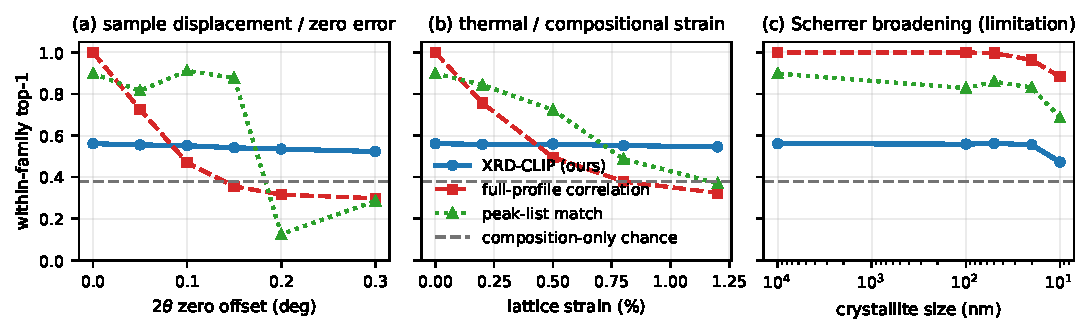
\includegraphics[width=\textwidth]{fig_sweeps.pdf}
  \caption{One-dial degradation of the query pattern (library stays
  clean-simulated). The learned embedding (blue) is flat under peak-position
  degradations---(a) $2\theta$ zero offset and (b) lattice strain---where
  full-profile correlation (red) collapses; it concedes (c) severe Scherrer
  broadening, the one position-preserving axis, to correlation. Grey dashed line
  is composition-only chance.}
  \label{fig:sweeps}
\end{figure*}

\begin{figure*}[t]
  \centering
  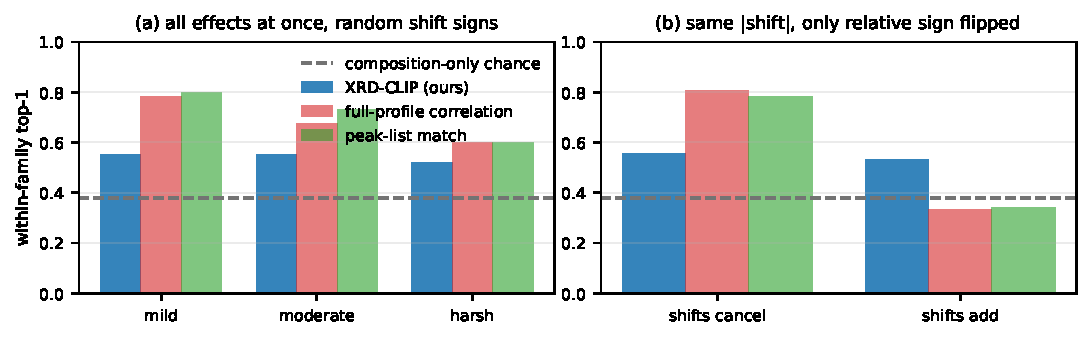
\includegraphics[width=\textwidth]{fig_combined.pdf}
  \caption{(a) All measurement effects applied at once with per-crystal random
  shift signs: the model (blue) stays near 0.55 mild$\to$harsh while both
  classical methods fall. (b) The sign-cancellation control: holding the shift
  \emph{magnitudes} fixed (0.10$^\circ$ displacement, 0.6\% strain) and flipping
  only the relative sign, correlation and peak-list drop from $\approx0.80$ to
  composition-only chance while the model holds.}
  \label{fig:combined}
\end{figure*}

\textbf{Peak-position degradations are where the model earns its keep.}
Figure~\ref{fig:sweeps} degrades one physical dial at a time, perturbing only the
query. Under a $2\theta$ zero offset (sample displacement), the model is flat
(0.561$\to$0.523) while full-profile correlation collapses (1.0$\to$0.298) and
overtakes both classical methods beyond 0.15$^\circ$. Under lattice strain the
model is again flat (0.561$\to$0.546) versus correlation (1.0$\to$0.323). These
two axes---sample displacement, thermal expansion, and zero/wavelength error---are
the real-world killers of search-match. The model's honest limitation is the one
position-\emph{preserving} axis: at a 10\,nm crystallite size, Scherrer broadening
smears peaks and correlation (0.884) beats the model (0.472).

\textbf{A sign-cancellation control isolates a genuine invariance.} Stacking every
dial at fixed same-sign values would be misleading: a positive displacement pushes
peaks up in $2\theta$ while cell expansion pushes them down, so at fixed
magnitudes the two partially cancel and \emph{artificially rescue} the correlation
baseline. Figure~\ref{fig:combined}(a) instead draws per-crystal random shift
signs on top of a fixed broadening/texture/noise/background base; the model holds
$0.554\to0.521$ mild$\to$harsh while correlation falls $0.782\to0.599$ and
peak-list $0.797\to0.601$. Figure~\ref{fig:combined}(b) is the control: fixing the
shift magnitudes and flipping only the relative sign, correlation drops from
\textbf{0.807} (cancel) to \textbf{0.334} (add) and peak-list from 0.784 to 0.340,
both at composition-only chance, while the model holds ($0.555\to0.534$). For the
$\sim$50\% of real samples where the two shifts reinforce, classical search-match
is no better than knowing the formula---and it cannot know in advance which half a
sample falls in. The learned embedding's invariance is sign-independent; the
baselines' apparent robustness is a coincidental cancellation.

\section{Ablations: emergent vs.\ learned robustness}\label{sec:ablation}
\begin{table}[t]
  \centering
  \caption{Ablating training-time augmentation (within-family top-1;
  composition-only chance $=0.380$). Two twins, identical architecture, data, and
  60-epoch schedule; only the augmentation changes.}
  \label{tab:ablation}
  \small
  \begin{tabular}{lccc}
    \toprule
     & full aug & no shift/strain & no aug \\
     & (main) & aug & (clean) \\
    \midrule
    clean within-family        & 0.561 & 0.553 & 0.557 \\
    pure shift @ 0.1$^\circ$   & 0.552 & 0.549 & 0.552 \\
    field (mild)               & 0.554 & 0.560 & 0.380 \\
    field (harsh)              & 0.521 & 0.528 & 0.379 \\
    sign: add                  & 0.534 & 0.530 & 0.379 \\
    \bottomrule
  \end{tabular}
\end{table}

Two ablations settle where the robustness comes from (Table~\ref{tab:ablation}).
\emph{First}, zeroing the shift and strain augmentation ranges while keeping the
rest (\textbf{no shift/strain aug}) changes nothing: the twin tracks the main
model within 1\% on every axis, including pure shift and the sign-add regime. Peak
position invariance is therefore \textbf{emergent}---a 1D CNN with global pooling
is intrinsically tolerant to peak translation, and small strain is locally
translation-like---not something the shift augmentation taught. \emph{Second},
removing \emph{all} augmentation and training on perfectly clean patterns
(\textbf{no aug}) is the decisive control. That twin still retrieves cleanly
(0.557) and is still flat under a pure shift (0.552 at 0.1$^\circ$), but it
\textbf{collapses to chance the moment any realistic instrument profile is
present}: full-field retrieval is $0.380/0.381/0.379$ (mild/moderate/harsh), and
the crystallite-size sweep alone walks it down $0.557\to0.410\to0.395\to0.390$
(100/50/20\,nm).

This is the direct answer to the natural objection---``isn't within-family
retrieval just simulated-fingerprint leakage, since the query is simulated from
the target?'' If it were, the clean-trained twin would retrieve fine under
realistic conditions. It does not: a clean-trained encoder cannot retrieve at all
once broadening, texture, noise, and background appear. The physics-grounded
augmentation is doing genuine simulation-to-realistic generalization;
measurement-profile robustness is \textbf{learned}, while peak-position invariance
is architectural.

\section{A sim-to-real spot check}\label{sec:realcheck}
Every result above evaluates the model on the same physics-based simulator it was
trained with. As an initial check of transfer beyond the simulator, we retrieved
three \emph{real} experimental PXRD patterns against the full 30{,}887-structure
test library, digitized point-by-point from the Rietveld powder-refinement data
deposited as supporting information with the structures' original
determination papers (Cu-K$\alpha_1$, matching our simulation exactly). For
racemic ibuprofen (IBPRAC04)~\cite{derollez2010ibuprofen}---whose structure is a
corpus entry, but whose \emph{real measured pattern} the model has never seen in
any form---the true structure ranks \textbf{1{,}872 of 30{,}887} by cosine
similarity (top 6.1\%): well above the library midpoint on a single real query,
though not top-1. For two real patterns of phenobarbital polymorphs Form
I/II~\cite{platteau2005phenobarbital}, the specific determination is not itself a
corpus structure (only sibling PHBARB polymorphs are), so no retrieval rank
applies; nearest-neighbour inspection surfaced no chemically plausible match,
underscoring that retrieval scoring requires the query's true structure to be a
library candidate. This is a small-$N$ spot check, not a systematic real-data
benchmark---scaling it to the tens of real molecular patterns available in the
powder-diffraction literature is the natural next step.

\section{Limitations}
The sim-to-real check above is a single-digit-$N$ spot check, not a systematic
benchmark; the bulk of our evaluation remains on the physics-grounded simulator,
for which our augmentation and the sign-cancellation control are designed as
diagnostics. The model concedes severe Scherrer broadening to full-profile
correlation, and within-family top-1 of 0.561, while well above the 0.380 chance
floor, leaves clear headroom---an explicit low-angle/wide-angle encoder
split~\cite{xu2025xccp} and light Rietveld reranking are natural next steps. Our
benchmark is molecular (CSD); the inorganic and MOF regimes are already served by
composition/symmetry-aware retrieval~\cite{xu2025xccp,lai2025xtalnet}.

\section{Conclusion}
Molecular polymorph discrimination is the regime where composition- and
symmetry-based PXRD retrieval is structurally blind, and it is exactly where a
pattern$\leftrightarrow$packing contrastive model earns its keep. On a
family-safe CSD benchmark the learned embedding resolves same-molecule siblings
above chance and, more importantly, holds its accuracy under the peak-position
perturbations that send classical search-match to chance---a sign-independent
invariance the classical methods cannot guarantee. Ablations show this robustness
is part architectural and part learned from physics-grounded augmentation, and is
not fingerprint leakage. The same contrastive retriever is the natural candidate
ranker for PXRD-conditioned generative crystal structure
prediction~\cite{lai2025xtalnet,johansen2025decifer} on molecular crystals, which
we leave to future work.

\bibliographystyle{IEEEtran}
\bibliography{refs}

\end{document}
